\documentclass[10pt,letterpaper]{article}

\usepackage[utf8]{inputenc}
\usepackage[T1]{fontenc}
\usepackage{microtype}
\usepackage{times}
\usepackage{amsmath,amssymb,bm,amsthm}
\usepackage{booktabs}
\usepackage{hyperref}
\usepackage[margin=1in]{geometry}
\usepackage{graphicx}
\usepackage{subcaption}

\newtheorem{theorem}{Theorem}
\newtheorem{lemma}{Lemma}
\newtheorem{corollary}{Corollary}
\theoremstyle{definition}
\newtheorem{assumption}{Assumption}
\newtheorem{definition}{Definition}

\title{On the Landscape Complexity Measure for Fully Connected ReLU Networks under Squared Loss}

\author{%
  Andrey Grabovoy\thanks{Correspondence to: \texttt{grabovoy@ipu.ru}}\\
  \textit{Institute of Control Sciences of the Russian Academy of Sciences, Moscow, Russia}
}

\date{\vspace{-0.5em}}

\begin{document}

\maketitle

\begin{abstract}
Loss-landscape analysis and classical uniform-complexity theory describe different aspects of neural models. Their relation in regression is still not fully explicit. This paper develops a \emph{Landscape Complexity Measure} for scalar regression with fully connected ReLU networks under squared loss. The measure is defined through the spectral dispersion of per-example Hessians around their empirical average. It is meant to capture local Hessian variability at a fixed reference parameter. For bias-free, norm-bounded fully connected networks, the paper adapts prior Hessian bounds to the mean-squared-error setting. It also identifies the simplification of the outer loss Hessian in the scalar-output case. Sample-growth arguments are used only as motivation for studying Hessian dispersion. The paper then derives scaling laws for the Landscape Complexity Measure in terms of depth, width, and norm constraints. It compares these laws with empirical Rademacher complexity for linear and two-layer predictors. The comparison shows a clear difference in role. The Landscape Complexity Measure reflects local geometric variability of the loss landscape. Empirical Rademacher complexity reflects global capacity of the predictor class. The theoretical comparison is summarized in one table. The paper also reports controlled numerical experiments whose trends are qualitatively consistent with the derived orders.
\end{abstract}

\noindent\textbf{Keywords:} landscape complexity measure; loss landscape; hessian dispersion; rademacher complexity; squared loss; scalar regression; fully connected ReLU networks.

\section{Introduction}

Deep neural networks are trained by solving high-dimensional nonconvex optimization problems. Because of this, the geometry of the loss landscape is important for understanding optimization and local stability \cite{fort2019emergent,ghorbani2019,sagun2018}.
At the same time, statistical learning theory studies model classes through capacity measures. These measures control the gap between empirical and population behavior \cite{bartlett2002,vapnik1998}.
For scalar regression with fully connected ReLU networks, both viewpoints matter. However, under squared loss, their relation is still not stated in a direct form centered on one complexity object \cite{bartlett2002,vapnik1998,kiselev2024hessian}.

Several ingredients are already available in the literature \cite{bartlett2002,ghorbani2019,kiselev2024hessian}.
Empirical and theoretical studies analyze Hessian spectra, curvature concentration, and structural properties of neural loss surfaces \cite{ghorbani2019,sagun2018,papyan2019hessian,wu2022dissecting,pennington2017}.
Classical complexity theory provides Rademacher, Gaussian, VC-dimension, and pseudodimension tools for controlling uniform deviations of neural function classes \cite{bartlett2002,vapnik1998,harvey2019jmlr}.
For fully connected ReLU architectures, prior Hessian-based work established spectral bounds in the cross-entropy setting. It also linked those bounds to sample-growth analysis of the empirical risk \cite{kiselev2024hessian}.

Yet the regression picture remains incomplete \cite{bartlett2002,vapnik1998,kiselev2024hessian}.
Uniform-capacity bounds describe the size of a hypothesis class. They do not directly measure how curvature varies across training examples at a fixed parameter \cite{bartlett2002,vapnik1998}.
Hessian-based analyses take the opposite viewpoint. They are local, and they are often developed for other losses or other tasks \cite{kiselev2024hessian,jacot2018ntk,lee2018wide}.
As a result, for scalar regression under squared loss, the role of per-example Hessian dispersion has not been isolated cleanly. It has also not been compared side by side with empirical Rademacher complexity for the same fully connected architectures \cite{bartlett2002,kiselev2024hessian}.

This paper addresses that gap by placing the \emph{Landscape Complexity Measure} at the center of the analysis \cite{kiselev2024hessian}.
The measure is defined through the dispersion of per-example Hessians around their empirical average. It is motivated by Hessian-based sample-growth analysis of the type developed in prior fully connected work \cite{kiselev2024hessian}.
The paper adapts prior fully connected Hessian bounds to the mean-squared-error setting. It uses sample-growth arguments only to explain why this Hessian-dispersion quantity is natural and informative \cite{kiselev2024hessian,skorski2019chain}.
This gives a regression-specific local complexity notion. It can be compared directly with empirical Rademacher complexity for the same model classes \cite{bartlett2002,vapnik1998,kiselev2024hessian}.

The results show how the Landscape Complexity Measure scales with depth, width, and norm constraints in bias-free fully connected networks. They also show how this scaling differs from that of empirical Rademacher complexity in linear and two-layer regimes \cite{bartlett2002,harvey2019jmlr,kiselev2024hessian}.
The paper also identifies the simplification specific to squared loss relative to the softmax template. It summarizes the theoretical orders in a comparative table. It complements the analysis with controlled numerical experiments whose trends are qualitatively consistent with the theory \cite{kiselev2024hessian}.
Overall, the paper develops the Landscape Complexity Measure as a regression-specific Hessian-dispersion quantity. It studies this quantity alongside classical uniform complexity for fully connected ReLU models \cite{bartlett2002,vapnik1998,kiselev2024hessian}.

\section{Related works}\label{sec:related}

Research on neural loss landscapes has developed in several directions. Qualitative studies of nonconvex surfaces emphasize local minima, saddle structure, and basin geometry \cite{choromanska2015,fort2019emergent}. Visualization-based work studies low-dimensional views of high-dimensional objectives \cite{li2018visualizing,fort2019large}. A more quantitative line focuses on Hessian spectra and curvature structure. Empirical studies often observe a bulk of near-zero eigenvalues together with a smaller set of dominant directions \cite{ghorbani2019,sagun2018,papyan2019hessian,wu2022dissecting}. Random-matrix and scaling perspectives relate such patterns to width, data randomness, and model size \cite{pennington2017,xie2022powerlaw}. Connections between geometry and generalization are also discussed through flat-versus-sharp minima and related stability viewpoints \cite{hochreiter1994,neyshabur2017exploring,dinh2017sharp}. For the present paper, this literature provides the geometric background. However, it does not by itself yield a single local complexity quantity tailored to squared-loss regression.

A second line of work studies neural models through global complexity measures. Classical results based on VC dimension, covering numbers, and Rademacher or Gaussian complexity control uniform deviations over hypothesis classes \cite{vapnik1998,bartlett2002}. For ReLU networks, pseudo-dimension and related combinatorial bounds refine the dependence on architecture and parameterization \cite{harvey2019jmlr}. These tools are fundamental for statistical learning theory. However, they quantify worst-case capacity of a function class. They do not describe variation of curvature across training examples at a fixed reference parameter. In that sense, they answer a different question from the local Hessian-dispersion viewpoint developed here.

Several nearby perspectives are also relevant, but they have a different emphasis. Neural tangent kernel and infinite-width analyses connect wide networks to kernel predictors and near-linearized training dynamics \cite{jacot2018ntk,lee2018wide}. However, they are not designed to quantify per-example Hessian dispersion at a chosen parameter value. On the technical side, tensor-calculus treatments of higher-order chain rules help organize Hessian decompositions in compositional models \cite{skorski2019chain}. Structural studies of Hessian maps clarify low-rank and layerwise phenomena in neural networks \cite{wu2022dissecting}. This line is used mainly as mathematical background for the regression-specific Hessian formulas that follow.

The closest predecessor to the present work is the Hessian-based analysis of fully connected ReLU classifiers in \cite{kiselev2024hessian}. There, per-example Hessians are controlled in spectral norm and linked to sample-growth estimates for the empirical risk under cross-entropy. Related Hessian-based arguments were also developed for convolutional, matricized architectures in \cite{meshkov2024ispras}. The present paper keeps the fully connected setting, but shifts the focus in three ways. The setting changes from classification to scalar regression. It also changes from cross-entropy to squared loss. In addition, the main endpoint changes from a sample-growth estimate to the \emph{Landscape Complexity Measure} itself. This makes it natural to compare the resulting local Hessian-dispersion quantity with empirical Rademacher complexity for the same linear and two-layer model classes.

\section{Problem statement}\label{sec:problem}

Let $(\mathbf{x},\mathbf{y})$ be i.i.d.\ on $\mathbb{R}^{n}\times\mathbb{R}$ with scalar targets $\mathbf{y}_i\in\mathbb{R}$.
Let
\[
  D = \{(\mathbf{x}_1,\mathbf{y}_1),\ldots,(\mathbf{x}_m,\mathbf{y}_m)\},
  \qquad |D|=m,
  \qquad \mathbf{x}_i\in\mathbb{R}^n .
\]
Let $f_{\boldsymbol{\theta}}:\mathbb{R}^{n}\to\mathbb{R}$ be an $L$-layer fully connected ReLU network,
$\boldsymbol{\theta}\in\mathbb{R}^P$. The main spectral Hessian bounds below will additionally assume a bias-free architecture together with uniform bounds on weights and inputs. The instantaneous squared loss is
\begin{equation}\label{eq:loss-i}
  \ell_i(\boldsymbol{\theta})
  = \ell\bigl(f_{\boldsymbol{\theta}}(\mathbf{x}_i),\mathbf{y}_i\bigr)
  = \tfrac{1}{2}\bigl(f_{\boldsymbol{\theta}}(\mathbf{x}_i)-y_i\bigr)^2,
  \qquad \mathbf{y}_i = y_i\in\mathbb{R}.
\end{equation}
The empirical risk on the first $k$ observations is
\begin{equation}\label{eq:Lk}
  \mathcal{L}_k(\boldsymbol{\theta}) = \frac{1}{k}\sum_{i=1}^{k} \ell\bigl(f_{\boldsymbol{\theta}}(\mathbf{x}_i),\mathbf{y}_i\bigr),
  \qquad k=1,\ldots,m .
\end{equation}

\section{Landscape complexity measure under squared loss}\label{sec:landscape}

This section formalizes the Landscape Complexity Measure under squared loss. It starts from the fully connected Hessian framework of \cite{kiselev2024hessian}.
The difference $\mathcal{L}_{k+1}-\mathcal{L}_k$ plays only an auxiliary role here. It gives one natural second-order route by which Hessian dispersion enters the analysis when the training set grows by one example.
A second-order approximation shows that the key term is controlled by the difference between the new-example Hessian and the average Hessian on the first $k$ examples. The \emph{landscape complexity measure}~\eqref{eq:muf} quantifies the typical size of that deviation in spectral norm.
The section first defines the landscape complexity measure $\mu_f$ and a mild stationarity condition at a reference point~$\boldsymbol{\theta}^*$. It then derives the sample-growth inequality~\eqref{eq:mod-diff} only as motivation for the appearance of $\mu_f$. Finally, it proves spectral estimates for $\|\mathbf{H}_i\|_2$ under uniform weight and input bounds and derives the scaling of~$\mu_f$.
Corollaries then record the linear and single-hidden-layer regimes.

\begin{definition}[Landscape complexity measure]\label{def:muf}
Let $\mathbf{H}_i(\boldsymbol{\theta}) = \nabla^2_{\boldsymbol{\theta}} \ell(f_{\boldsymbol{\theta}}(\mathbf{x}_i),\mathbf{y}_i)$.
The \emph{landscape complexity measure} is
\begin{equation}\label{eq:muf}
  \mu_f(f\mid D)
  = \mathsf{E}_{\mathbf{x}_i\in D}\left\|
      \mathbf{H}_{i}(\boldsymbol{\theta}^*)
      - \mathsf{E}_{\mathbf{x}_i\in D}\mathbf{H}_{i}(\boldsymbol{\theta}^*)
    \right\|_2 ,
\end{equation}
where $\mathsf{E}_{\mathbf{x}_i\in D}$ denotes expectation with respect to a uniform index on $D$ for a fixed reference $\boldsymbol{\theta}^*$.
Thus $\mu_f$ is large when per-example Hessians disagree in operator norm around their mean on~$D$.
\end{definition}
\noindent
For ReLU networks, the Hessian expressions below are understood on regions of parameter space where the activation pattern of each observed input is fixed. Such regions cover parameter space up to measure-zero kink boundaries, so the displayed derivatives are interpreted almost everywhere in~$\boldsymbol{\theta}$ and, in particular, at reference points~$\boldsymbol{\theta}^*$ where these derivatives exist.

\begin{assumption}[Approximate stationarity at $\boldsymbol{\theta}^*$]\label{ass:local-min}
For some $\varepsilon_g\ge 0$,
\begin{equation}\label{eq:eps-g}
  \bigl\|\nabla \mathcal{L}_k(\boldsymbol{\theta}^*)\bigr\|_2 \le \varepsilon_g,
  \qquad
  \bigl\|\nabla \mathcal{L}_{k+1}(\boldsymbol{\theta}^*)\bigr\|_2 \le \varepsilon_g .
\end{equation}
\end{assumption}
\noindent
Small gradients at $\boldsymbol{\theta}^*$ are allowed instead of requiring exact critical points. The case $\varepsilon_g=0$ recovers the stationary setting emphasized in related work.

Let $\mathbf{H}^{(k)}(\boldsymbol{\theta})=\frac{1}{k}\sum_{i=1}^{k}\mathbf{H}_i(\boldsymbol{\theta})$.
On regions where the relevant derivatives exist, a second-order approximation of $\mathcal{L}_{k+1}$ and $\mathcal{L}_k$ around $\boldsymbol{\theta}^*$ isolates three contributions. The first is a zeroth-order term coming from the change in average loss. The second is a quadratic term driven by $\mathbf{H}^{(k+1)}-\mathbf{H}^{(k)}$. The third consists of linear remainders controlled by the gradient bounds~\eqref{eq:eps-g}.
Under Assumption~\ref{ass:local-min}, this motivates the local proxy estimate discussed in Appendix~\ref{app:proof-mod-diff}:
\begin{align}\label{eq:mod-diff}
  \bigl|\mathcal{L}_{k+1}(\boldsymbol{\theta}) - \mathcal{L}_k(\boldsymbol{\theta})\bigr|
  &\le \frac{1}{k+1}
  \left|
    \ell(f_{\boldsymbol{\theta}^*}(\mathbf{x}_{k+1}),\mathbf{y}_{k+1})
    - \frac{1}{k}\sum_{i=1}^{k}\ell(f_{\boldsymbol{\theta}^*}(\mathbf{x}_{i}),\mathbf{y}_{i})
  \right|
  \nonumber\\
  &\quad + \frac{\|\boldsymbol{\theta}-\boldsymbol{\theta}^*\|_2^2}{k+1}
  \left\| \mathbf{H}_{k+1}(\boldsymbol{\theta}^*) - \frac{1}{k}\sum_{i=1}^{k}\mathbf{H}_{i}(\boldsymbol{\theta}^*) \right\|_2
  + 2\,\varepsilon_g\,\|\boldsymbol{\theta}-\boldsymbol{\theta}^*\|_2 .
\end{align}
Equation~\eqref{eq:mod-diff} is used only as a local approximation-based proxy. It links sample growth to Hessian dispersion, but it is not a standalone exact identity.
The middle line is the bridge to~\eqref{eq:muf}. Bounding $\|\mathbf{H}_{k+1}-\frac{1}{k}\sum_{i\le k}\mathbf{H}_i\|_2$ is closely related to controlling dispersion of per-example Hessians around an empirical average.

Let $u=f_{\boldsymbol{\theta}}(\mathbf{x})$. For squared loss, $\partial^2 \ell/\partial u^2=1$; for softmax
cross-entropy, $\|\partial^2 \ell/\partial \mathbf{u}^2\|_2\le\sqrt{2}$ at the logits $\mathbf{u}$
\cite{kiselev2024hessian}.
The chain-rule decomposition of $\mathbf{H}_i$ follows \cite{kiselev2024hessian}, Section~3.4. For scalar output, it reduces to a sum of a Gauss--Newton--type term and a term weighted by the loss gradient; see Appendix~\ref{app:proof-lemma-hess}.
The next lemma gives a concrete $M_{\mathbf{H}}$ for bias-free fully connected ReLU nets under spectral constraints on weights and inputs. This expression is obtained by specializing the $K$-label bound of \cite{kiselev2024hessian}, Theorem~1, to scalar output and squared loss.

\begin{lemma}[Spectral norm of the per-example Hessian for squared loss and FC networks]\label{lem:hess-mse}
Consider a bias-free FC ReLU network with
$\|\mathbf{W}^{(p)}\|_2 \le M_{\mathbf{W}}$, $\|\mathbf{x}_i\|_2 \le M_{\mathbf{x}}$ for all $p$ and $i$.
Then there exists a constant $M_{\mathbf{H}}$ such that for every $i$ and for every parameter point where the required derivatives exist,
\begin{equation}\label{eq:Mh-bound}
  \bigl\| \mathbf{H}_i(\boldsymbol{\theta}) \bigr\|_2 \le M_{\mathbf{H}}
  := L\, M_{\mathbf{x}}^2 M_{\mathbf{W}}^{2L}
  + \sum_{s=1}^{L} M_{\mathbf{W}}^{2s} .
\end{equation}
If $|w_{ij}^{(p)}|\le M$ on $h\times h$ blocks, then $M_{\mathbf{W}}\le hM$ and
$\|\mathbf{H}_i(\boldsymbol{\theta})\|_2 = O\!\bigl(L(hM)^{2L}\bigr)$ asymptotically.
\end{lemma}
\noindent\textit{Proof.} See Appendix~\ref{app:proof-lemma-hess}.

As a by-product, the local proxy estimate~\eqref{eq:mod-diff}, together with either the uniform Hessian bound from Lemma~\ref{lem:hess-mse} or the exact MSE interpolation identity~\eqref{eq:hess-mse-decomp}, gives an $O(1/k)$ contribution to $|\mathcal{L}_{k+1}-\mathcal{L}_k|$. The separate stationarity term proportional to~$\varepsilon_g$ does not vanish in general.

\begin{theorem}[Local landscape increment bound for the squared loss with FC networks]\label{thm:landscape-mse}
Let $\boldsymbol{\theta}$ satisfy $\|\boldsymbol{\theta}-\boldsymbol{\theta}^*\|_2\le R$.
Assume $\bigl|\ell(f_{\boldsymbol{\theta}^*}(\mathbf{x}_i),\mathbf{y}_i)\bigr|\le M_{\ell}$ for all $i$, that Lemma~\ref{lem:hess-mse} applies at $\boldsymbol{\theta}^*$, and that Assumption~\ref{ass:local-min} holds with some $\varepsilon_g\ge 0$.
Then, conditional on the local proxy estimate~\eqref{eq:mod-diff},
\begin{equation}\label{eq:thm-bound}
  \bigl|\mathcal{L}_{k+1}(\boldsymbol{\theta}) - \mathcal{L}_k(\boldsymbol{\theta})\bigr|
  \le \frac{2}{k+1}\bigl( M_{\ell} + M_{\mathbf{H}} R^2 \bigr) + 2\,\varepsilon_g\, R .
\end{equation}
This is the worst-case bound obtained from uniform Hessian control within the local proxy framework. Under the asymptotics of $M_{\mathbf{H}}$, the curvature contribution has order
\begin{equation}\label{eq:rate}
  \bigl|\mathcal{L}_{k+1}(\boldsymbol{\theta}) - \mathcal{L}_k(\boldsymbol{\theta})\bigr|
  \;=\; O\!\left(\frac{L(hM)^{2L} R^2}{k}\right)
\end{equation}
as in \cite{kiselev2024hessian}, Lemma~2.

The next part records a residual-aware refinement.
If, moreover,
\[
  \bigl|f_{\boldsymbol{\theta}^*}(\mathbf{x}_i)-y_i\bigr|\le \varepsilon_y,
  \qquad i=1,\dots,m,
\]
and each observed input stays in a fixed activation region in a neighborhood of $\boldsymbol{\theta}^*$, define
\[
  \mathbf{g}_i:=\nabla_{\boldsymbol{\theta}}f_{\boldsymbol{\theta}^*}(\mathbf{x}_i),
  \qquad
  M_{\nabla^2 f}:=
  \max_{1\le i\le m}\bigl\|\nabla_{\boldsymbol{\theta}}^2 f_{\boldsymbol{\theta}^*}(\mathbf{x}_i)\bigr\|_2 .
\]
Then
\begin{equation}\label{eq:interp-hessian}
  \bigl\|
    \mathbf{H}_i(\boldsymbol{\theta}^*)
    - \mathbf{g}_i\mathbf{g}_i^\top
  \bigr\|_2
  \le \varepsilon_y M_{\nabla^2 f}
\end{equation}
for every $i$, and
\begin{equation}\label{eq:muf-interp-general}
  \mu_f(f\mid D)\le
  2\max_{1\le i\le m}\|\mathbf{g}_i\|_2^2
  + 2\varepsilon_y M_{\nabla^2 f} .
\end{equation}
Consequently,
\begin{equation}\label{eq:thm-bound-interp}
  \bigl|\mathcal{L}_{k+1}(\boldsymbol{\theta}) - \mathcal{L}_k(\boldsymbol{\theta})\bigr|
  \le
  \frac{\varepsilon_y^2 + 2R^2\bigl(\max_{1\le i\le m}\|\mathbf{g}_i\|_2^2 + \varepsilon_y M_{\nabla^2 f}\bigr)}{k+1}
  + 2\,\varepsilon_g\,R .
\end{equation}
If in addition $\|\mathbf{W}^{(p)\star}\|_2\le M_{\mathbf{W}}$ for every layer and $\|\mathbf{x}_i\|_2\le M_{\mathbf{x}}$ for all $i$, then
\begin{equation}\label{eq:grad-interp-general}
  \max_{1\le i\le m}\|\mathbf{g}_i\|_2^2
  \le L M_{\mathbf{x}}^2 M_{\mathbf{W}}^{2L-2},
\end{equation}
hence
\begin{equation}\label{eq:rate-interp}
  \bigl|\mathcal{L}_{k+1}(\boldsymbol{\theta}) - \mathcal{L}_k(\boldsymbol{\theta})\bigr|
  \le
  \frac{\varepsilon_y^2 + 2R^2\bigl(L M_{\mathbf{x}}^2 M_{\mathbf{W}}^{2L-2} + \varepsilon_y M_{\nabla^2 f}\bigr)}{k+1}
  + 2\,\varepsilon_g\,R .
\end{equation}
In this neighborhood, $f_{\boldsymbol{\theta}}$ is twice differentiable on the observed inputs. The special case $\varepsilon_y=0$ recovers exact interpolation and reduces~\eqref{eq:interp-hessian} to the Gauss--Newton identity.
\end{theorem}
\noindent\textit{Proof.} See Appendix~\ref{app:proof-thm-landscape}.

The next results record the linear and shallow cases. Corollary~\ref{cor:muf} then summarizes the scaling of $\mu_f$ implied by Lemma~\ref{lem:hess-mse}.
For one hidden layer one has $L=2$, so the factor $(hM)^{2L}$ in the generic bound becomes $(hM)^4$ when the input bound is treated as fixed and absorbed into the implicit constants.

\begin{corollary}[Linear model]\label{cor:linear}\label{sec:particular}
If $f_{\boldsymbol{\theta}}(\mathbf{x})=\mathbf{w}^{\top}\mathbf{x}$ with $\boldsymbol{\theta}=\mathbf{w}\in\mathbb{R}^{n}$ and the same squared loss~\eqref{eq:loss-i}, then
$\mathbf{H}_i(\boldsymbol{\theta})=\mathbf{x}_i\mathbf{x}_i^{\top}$, which is independent of $\mathbf{w}$ and $y_i$, hence
$\|\mathbf{H}_i\|_2=\|\mathbf{x}_i\|_2^2$.
Under $\|\mathbf{x}_i\|_2\le M_{\mathbf{x}}$, one may take $M_{\mathbf{H}}=M_{\mathbf{x}}^2$ in Lemma~\ref{lem:hess-mse} and Corollary~\ref{cor:muf} by replacing the ReLU-network bound with this rank-one Hessian.
The landscape complexity measure~\eqref{eq:muf} is then governed by the dispersion of the rank-one matrices $\mathbf{x}_i\mathbf{x}_i^{\top}$ around their sample average.
\end{corollary}

\begin{corollary}[Single hidden layer, FC ReLU]\label{cor:shallow}
Consider one hidden layer of width $h$: $\mathbb{R}^{n}\to\mathbb{R}^{h}\to\mathbb{R}$ with ReLU and bias-free weight matrices satisfying the same spectral bounds as in Lemma~\ref{lem:hess-mse}.
In the notation of Corollary~\ref{cor:muf}, this is the case $L=2$, so~\eqref{eq:muf-scale} yields the upper bound $\mu_f(f\mid D)=O((hM)^{4})$, in contrast to deeper networks where the factor $(hM)^{2L}$ grows faster in $L$.
Separately, if at a reference $\boldsymbol{\theta}^\star$ the pointwise residuals are uniformly small,
$\bigl|f_{\boldsymbol{\theta}^\star}(\mathbf{x}_i)-y_i\bigr|\le\varepsilon_y$ for all~$i$, then the residual-aware part of Theorem~\ref{thm:landscape-mse} and its exact identity~\eqref{eq:interp-hessian} yield the bound~\eqref{eq:muf-interp-general} on $\mu_f(f\mid D)$; under entrywise bounds this refines the worst-case $O(h^4)$.
\end{corollary}

\noindent
Lemma~\ref{lem:hess-mse} also implies an order for the landscape complexity measure~\eqref{eq:muf} in terms of depth, width, and norm bounds.

\begin{corollary}[Landscape complexity scaling]\label{cor:muf}
Under Lemma~\ref{lem:hess-mse}, together with entrywise bounds $|w_{ij}^{(p)}|\le M$ on the relevant $h\times h$ weight blocks and with the input bound $M_{\mathbf{x}}$ treated as fixed, the measure~\eqref{eq:muf} satisfies
\begin{equation}\label{eq:muf-scale}
  \mu_f(f\mid D) \;=\; O\!\bigl(L\,(hM)^{2L}\bigr),
\end{equation}
where $h$ denotes hidden width, $L$ depth, and $M$ an entrywise weight bound; the input bound $M_{\mathbf{x}}$ is absorbed into the implicit constant.
\end{corollary}

\section{Asymptotic scaling of the landscape complexity measure and Rademacher complexity}\label{sec:compare}

Section~\ref{sec:landscape} recorded local-proxy bounds for the empirical-risk increment. It also gave upper bounds for the landscape complexity measure $\mu_f(f\mid D)$ for fully connected maps.
This section places those orders next to classical \emph{uniform} complexity. The empirical Rademacher complexity~\eqref{eq:Rad-emp} measures how much a real-valued function class can correlate with random signs on the observed inputs, uniformly over the class~\cite{bartlett2002}.
The comparison is deliberately parallel. The same architectures and the same squared loss~\eqref{eq:loss-i} are used. However, the two notions answer different questions. The landscape complexity measure $\mu_f$ is tied to second-order dispersion of per-example Hessians at a reference parameter. In contrast, $\hat{\mathfrak{R}}_m$ is tied to the size and Lipschitz structure of the predictor family.
This section gives closed-form or generic upper bounds for $\hat{\mathfrak{R}}_m$. It also derives matching upper-order estimates for the landscape complexity measure $\mu_f$ from Section~\ref{sec:landscape}. Table~\ref{tab:compare-two} summarizes the contrast.

\begin{definition}[Empirical Rademacher complexity]\label{def:rademacher}
Let $\mathcal{F}$ be a class of functions $f:\mathbb{R}^n\to\mathbb{R}$.
Given $D$, the \emph{empirical Rademacher complexity} is
\begin{equation}\label{eq:Rad-emp}
  \hat{\mathfrak{R}}_m(\mathcal{F})
  := \mathbb{E}_{\boldsymbol{\sigma}}
  \left[
    \sup_{f\in\mathcal{F}}
    \frac{1}{m}\sum_{i=1}^{m}\sigma_i\, f(\mathbf{x}_i)
  \right],
\end{equation}
where $\sigma_1,\ldots,\sigma_m$ are i.i.d.\ Rademacher variables.
\end{definition}
\noindent
Below, $\mathcal{F}$ denotes the class of real-valued predictors $f_{\boldsymbol{\theta}}$ for each architecture; the comparison is between $\hat{\mathfrak{R}}_m(\mathcal{F})$ and $\mu_f(f\mid D)$ built from Hessians of the same maps at a reference~$\boldsymbol{\theta}^*$.

\subsection{Linear model}\label{subsec:linear-comp}

The linear class is the simplest setting: per-example Hessians are rank-one matrices $\mathbf{x}_i\mathbf{x}_i^{\top}$, so both $\hat{\mathfrak{R}}_m$ and $\mu_f$ admit elementary expressions in terms of the inputs.
Consider the class of linear predictors
\begin{equation}\label{eq:F-lin}
  \mathcal{F}_{\mathrm{lin}}(W)
  := \bigl\{ f_{\mathbf{w}}:\mathbf{x}\mapsto \mathbf{w}^{\top}\mathbf{x} \;\big|\; \|\mathbf{w}\|_2\le W \bigr\}.
\end{equation}
The radius $W$ is the natural partner to the weight norms that appear in Lemma~\ref{lem:hess-mse} when $L=1$.

For the empirical Rademacher complexity, by Cauchy--Schwarz,
$\frac{1}{m}\sum_i \sigma_i \mathbf{w}^{\top}\mathbf{x}_i
= \mathbf{w}^{\top}\bigl(\frac{1}{m}\sum_i \sigma_i \mathbf{x}_i\bigr)
\le W \bigl\|\frac{1}{m}\sum_{i=1}^{m}\sigma_i \mathbf{x}_i\bigr\|_2$,
and equality is attained at $\mathbf{w}$ parallel to $\sum_i \sigma_i \mathbf{x}_i$ whenever $\|\mathbf{w}\|_2=W$.
Hence
\begin{equation}\label{eq:Rad-lin-exact}
  \hat{\mathfrak{R}}_m(\mathcal{F}_{\mathrm{lin}}(W))
  = \frac{W}{m}\,
  \mathbb{E}_{\boldsymbol{\sigma}}\left\|
    \sum_{i=1}^{m}\sigma_i \mathbf{x}_i
  \right\|_2 .
\end{equation}
If $\|\mathbf{x}_i\|_2\le r$ for all $i$, then
$\mathbb{E}_{\boldsymbol{\sigma}}\|\sum_{i=1}^{m}\sigma_i \mathbf{x}_i\|_2^2=\sum_{i=1}^{m}\|\mathbf{x}_i\|_2^2$
and Jensen's inequality gives
$\mathbb{E}_{\boldsymbol{\sigma}}\|\sum_{i=1}^{m}\sigma_i \mathbf{x}_i\|_2 \le \bigl(\sum_{i=1}^{m}\|\mathbf{x}_i\|_2^2\bigr)^{1/2}$,
so
\begin{equation}\label{eq:Rad-lin-bound}
  \hat{\mathfrak{R}}_m(\mathcal{F}_{\mathrm{lin}}(W))
  \le \frac{W}{m}\left(\sum_{i=1}^{m}\|\mathbf{x}_i\|_2^2\right)^{1/2}
  \le \frac{W r}{\sqrt{m}} .
\end{equation}
If, in addition, coordinates are comparable in scale so that $\|\mathbf{x}_i\|_2^2=\Theta(n)$ uniformly in $i$ as $n\to\infty$, then the upper bound in~\eqref{eq:Rad-lin-bound} is of order $W\sqrt{n/m}$.

Covering-number and pseudo-dimension arguments for norm-bounded linear predictors also yield linear-in-$n$ complexity scaling in the ambient dimension under standard encodings \cite{bartlett2002,vapnik1998}. This matches the order of the upper estimate for $\mu_f$ in~\eqref{eq:muf-lin-mu}. The main comparison below is between~\eqref{eq:muf-lin-mu} and~\eqref{eq:Rad-lin-bound}.

For the Landscape Complexity Measure, Corollary~\ref{cor:linear} gives $\mathbf{H}_i=\mathbf{x}_i\mathbf{x}_i^{\top}$; let $\bar{\mathbf{H}}:=\frac{1}{m}\sum_{j=1}^{m}\mathbf{x}_j\mathbf{x}_j^{\top}$.
Then
\begin{equation}\label{eq:muf-lin-bound}
  \bigl\|\mathbf{H}_i-\bar{\mathbf{H}}\bigr\|_2
  \le \|\mathbf{x}_i\|_2^2 + \bigl\|\bar{\mathbf{H}}\bigr\|_2
  \le \|\mathbf{x}_i\|_2^2 + \frac{1}{m}\sum_{j=1}^{m}\|\mathbf{x}_j\|_2^2 ,
\end{equation}
using convexity of $\|\cdot\|_2$ for the second term.
Thus
\begin{equation}\label{eq:muf-lin-mu}
  \mu_f(f\mid D)
  \le 2\max_{1\le i\le m}\|\mathbf{x}_i\|_2^2
\end{equation}
for this linear model; the same averaging argument underlies Corollary~\ref{cor:muf}.
If $\|\mathbf{x}_i\|_2^2=\Theta(n)$ as $n\to\infty$, then~\eqref{eq:muf-lin-mu} implies the upper estimate $\mu_f(f\mid D)=O(n)$ up to the max over $i$.

Under the same input scaling, $\mu_f$ admits the upper estimate $O(n)$ by~\eqref{eq:muf-lin-mu}, while $\hat{\mathfrak{R}}_m$ in~\eqref{eq:Rad-lin-bound} is bounded by a quantity of order $W\sqrt{n/m}$.

\subsection{Two-layer fully connected ReLU network}\label{subsec:two-layer-comp}

A nonlinear class with one hidden layer is considered next. This matches Corollary~\ref{cor:shallow} and Lemma~\ref{lem:hess-mse} at depth $L=2$.
The upper scaling estimate $\mu_f=O((hM)^4)$ from~\eqref{eq:muf-scale} already differs sharply from the linear case. The natural question is how it compares to norm-based Rademacher estimates, which grow polynomially in~$h$ but also contain a $m^{-1/2}$ factor.

Consider one hidden layer of width $h$, with $\sigma=\mathrm{ReLU}$, bias-free weights, and
$f_{\boldsymbol{\theta}}(\mathbf{x})=\mathbf{w}^{(2)\top}\sigma\bigl(\mathbf{W}^{(1)}\mathbf{x}\bigr)$.
In the notation of Section~\ref{sec:landscape}, this is depth $L=2$ in Lemma~\ref{lem:hess-mse}.

For the empirical Rademacher complexity, let $\mathcal{F}_h$ denote the above class under constraints
$\|\mathbf{W}^{(1)}\|_2\le M_{\mathbf{W}}$ and $\|\mathbf{w}^{(2)}\|_2\le M_{\mathbf{W}}$, or under entrywise bounds $|w_{ij}|\le M$ as in Lemma~\ref{lem:hess-mse}.
Vector-contraction and norm-based bounds~\cite{bartlett2002} yield estimates of the form
\begin{equation}\label{eq:Rad-nn-generic}
  \hat{\mathfrak{R}}_m(\mathcal{F}_h)
  \;\lesssim\;
  \frac{C(\boldsymbol{\theta})}{m}\,
  \mathbb{E}_{\boldsymbol{\sigma}}\left\|
    \sum_{i=1}^{m}\sigma_i \mathbf{x}_i
  \right\|_2
  \;\lesssim\;
  \frac{C(\boldsymbol{\theta})\, r}{\sqrt{m}},
\end{equation}
where $C(\boldsymbol{\theta})$ depends on operator norms or Frobenius norms of $\mathbf{W}^{(1)}$ and $\mathbf{w}^{(2)}$ and grows at most polynomially in $h$ under fixed per-entry bounds $|w_{ij}|\le M$.
Thus the Rademacher term is $O(m^{-1/2})$ in sample size and, for fixed $M$ and bounded inputs, $O(\mathrm{poly}(h)/\sqrt{m})$ in width.
Uniform bounds based on covering numbers or fat-shattering for piecewise-linear networks also scale with parameter count and depth~\cite{bartlett2002,harvey2019jmlr}; these bounds are not developed here, and~\eqref{eq:Rad-nn-generic} is kept as the main classical counterpart to~$\mu_f$.

For the Landscape Complexity Measure, Corollary~\ref{cor:shallow} and~\eqref{eq:muf-scale} with $L=2$ give the upper bound $\mu_f(f\mid D)=O((hM)^{4})$.
For fixed $M$, this yields the worst-case estimate $\mu_f=O(h^4)$ as $h\to\infty$, whereas the Rademacher upper bound above is $O(\mathrm{poly}(h)/\sqrt{m})$ with a lower degree in $h$ under typical norm constraints.

The rate $O(h^4)$ is a \emph{uniform worst-case} consequence of Lemma~\ref{lem:hess-mse} and does not exploit the special structure of the squared loss in a small-residual regime.
When the residuals satisfy $|f_{\boldsymbol{\theta}^*}(\mathbf{x}_i)-y_i|\le \varepsilon_y$, the second term in the decomposition~\eqref{eq:hess-mse-decomp} is controlled by~$\varepsilon_y$ and the refinement in Theorem~\ref{thm:landscape-mse} applies.
For a two-layer network with $|w_{ij}|\le M$,
\[
  \left\|\nabla_{\boldsymbol{\theta}}f_{\boldsymbol{\theta}^*}(\mathbf{x}_i)\right\|_2^2
  = \sum_{j=1}^{h}\sigma\!\bigl((\mathbf{w}^{(1)\star}_j)^{\top}\mathbf{x}_i\bigr)^2
    + \sum_{j=1}^{h}(w_j^{(2)\star})^2 a_{ij}\|\mathbf{x}_i\|_2^2
  \le hM^2\bigl(\|\mathbf{x}_i\|_1^2+\|\mathbf{x}_i\|_2^2\bigr),
\]
where $a_{ij}=\mathbf{1}\{(\mathbf{w}^{(1)\star}_j)^\top \mathbf{x}_i>0\}$.
Substituting into~\eqref{eq:muf-interp-general} gives
\[
  \mu_f(f\mid D)
  \le 2hM^2\max_{1\le i\le m}\bigl(\|\mathbf{x}_i\|_1^2+\|\mathbf{x}_i\|_2^2\bigr)
     + 2\varepsilon_y M_{\nabla^2 f}.
\]
In particular, if $\|\mathbf{x}_i\|_2^2=\Theta(n)$ and $\|\mathbf{x}_i\|_1=\Theta(n)$ uniformly in~$i$, then
$\mu_f(f\mid D)=O(hM^2n^2 + \varepsilon_y M_{\nabla^2 f})$; when $\varepsilon_y$ is small and $n\asymp h$, the leading term is $O(M^2h^3)$.

For fixed $M$ and bounded inputs, the worst-case order from Corollary~\ref{cor:shallow} and~\eqref{eq:muf-scale} is $O(h^4)$, while the residual-aware part of Theorem~\ref{thm:landscape-mse} shows that in a small-residual MSE regime the scaling can improve to $O(hM^2n^2 + \varepsilon_y M_{\nabla^2 f})$ under entrywise bounds.
The Rademacher term in~\eqref{eq:Rad-nn-generic} remains $O(\mathrm{poly}(h)/\sqrt{m})$ because it is a uniform capacity quantity for the class rather than a local curvature quantity at~$\boldsymbol{\theta}^\star$.

Table~\ref{tab:compare-two} collects the worst-case growth orders for $\mu_f$ and $\hat{\mathfrak{R}}_m$ in the linear and two-layer regimes under the assumptions stated in this section; Theorem~\ref{thm:landscape-mse} records the sharper residual-aware refinement for MSE within the same local analysis.

\begin{table}[t]
\centering
\caption{Theoretical upper-order scaling of $\mu_f$ and empirical Rademacher complexity for the linear model and the two-layer FC ReLU under squared loss. For two-layer $\mu_f$, worst-case spectral bounds contrast with the residual-aware estimate from Theorem~\ref{thm:landscape-mse}; the latter comes from the local residual-aware analysis around~$\boldsymbol{\theta}^*$.}
\label{tab:compare-two}
\small
\setlength{\tabcolsep}{5pt}
\begin{tabular}{@{}p{0.19\linewidth}p{0.38\linewidth}p{0.38\linewidth}@{}}
\toprule
 & Linear & Two-layer FC ReLU \\
\midrule
$\mu_f(f\mid D)$ &
$O(n)$&
$O((hM)^4)$ in worst-case, and $O(hM^2n^2+\varepsilon_y M_{\nabla^2 f})$ in residual-aware \\
\addlinespace[0.35em]
$\hat{\mathfrak{R}}_m$ &
$O(W\sqrt{n/m})$ &
$O(\mathrm{poly}(h)/\sqrt{m})$ \\
\bottomrule
\end{tabular}
\end{table}

\section{Numerical comparisons with Rademacher complexity}\label{sec:experiments}

Table~\ref{tab:compare-two} records the asymptotic orders. For two-layer $\mu_f$, it includes both the worst-case and residual-aware cases.
This numerical section focuses on the comparative behavior of $\mu_f$ and $\hat{\mathfrak{R}}_m$. It does not attempt a direct validation of the auxiliary sample-growth bound for $\mathcal{L}_{k+1}-\mathcal{L}_k$.
The study evaluates $\mu_f(f\mid D)$ and the empirical Rademacher complexity~\eqref{eq:Rad-emp} in three controlled settings. These are: linear predictors with a sweep in ambient dimension~$n$; linear predictors with a sweep in sample size~$m$; and a two-layer FC ReLU with a sweep in hidden width~$h$ under entrywise bounds and planted worst-case data.

\paragraph{Common details.}
For each experiment, repeated draws of the data-generating process are averaged using independent seeds. Where appropriate, the mean together with one standard deviation is plotted as a shaded band.
For $\mathcal{F}_{\mathrm{lin}}(W)$, the Rademacher supremum in~\eqref{eq:Rad-emp} reduces to the closed form behind~\eqref{eq:Rad-lin-exact}--\eqref{eq:Rad-lin-bound}. The expectation over $\boldsymbol{\sigma}$ is approximated by Monte Carlo with $4096$ draws.
For the two-layer class, the supremum over $\boldsymbol{\theta}$ is approximated by projected gradient ascent on the entrywise ball, using the same $M$ as in the construction. Each estimate uses $n_{\sigma}$ Rademacher draws. The optimizer and iteration budget are listed in the notebook.

\paragraph{Linear model, sweep in $n$ (fixed $m$).}
Inputs are drawn from the synthetic linear dataset described in the code (Gaussian rows with randomized radii, scalar Gaussian noise on targets).
The setup fixes $m=256$ and varies $n$ along an evenly spaced grid from $8$ to $128$ with 12 values. For each $(n,m)$, $\mu_f$ is computed from the rank-one Hessians $\mathbf{H}_i=\mathbf{x}_i\mathbf{x}_i^\top$ as in Subsection~\ref{subsec:linear-comp}, and $\hat{\mathfrak{R}}_m(\mathcal{F}_{\mathrm{lin}}(W))$ is computed with $W=2$.
The experiment uses $16$ random trials per~$n$.
Figure~\ref{fig:exp01} uses two vertical axes on log scales. This keeps $\mu_f$ and $\hat{\mathfrak{R}}_m$ readable on the same plot. The figure shows that $\mu_f$ grows roughly linearly in~$n$, while $\hat{\mathfrak{R}}_m$ grows like $\sqrt{n}$ at fixed~$m$. This matches the contrast in Table~\ref{tab:compare-two}.

\begin{figure}[t]
\centering
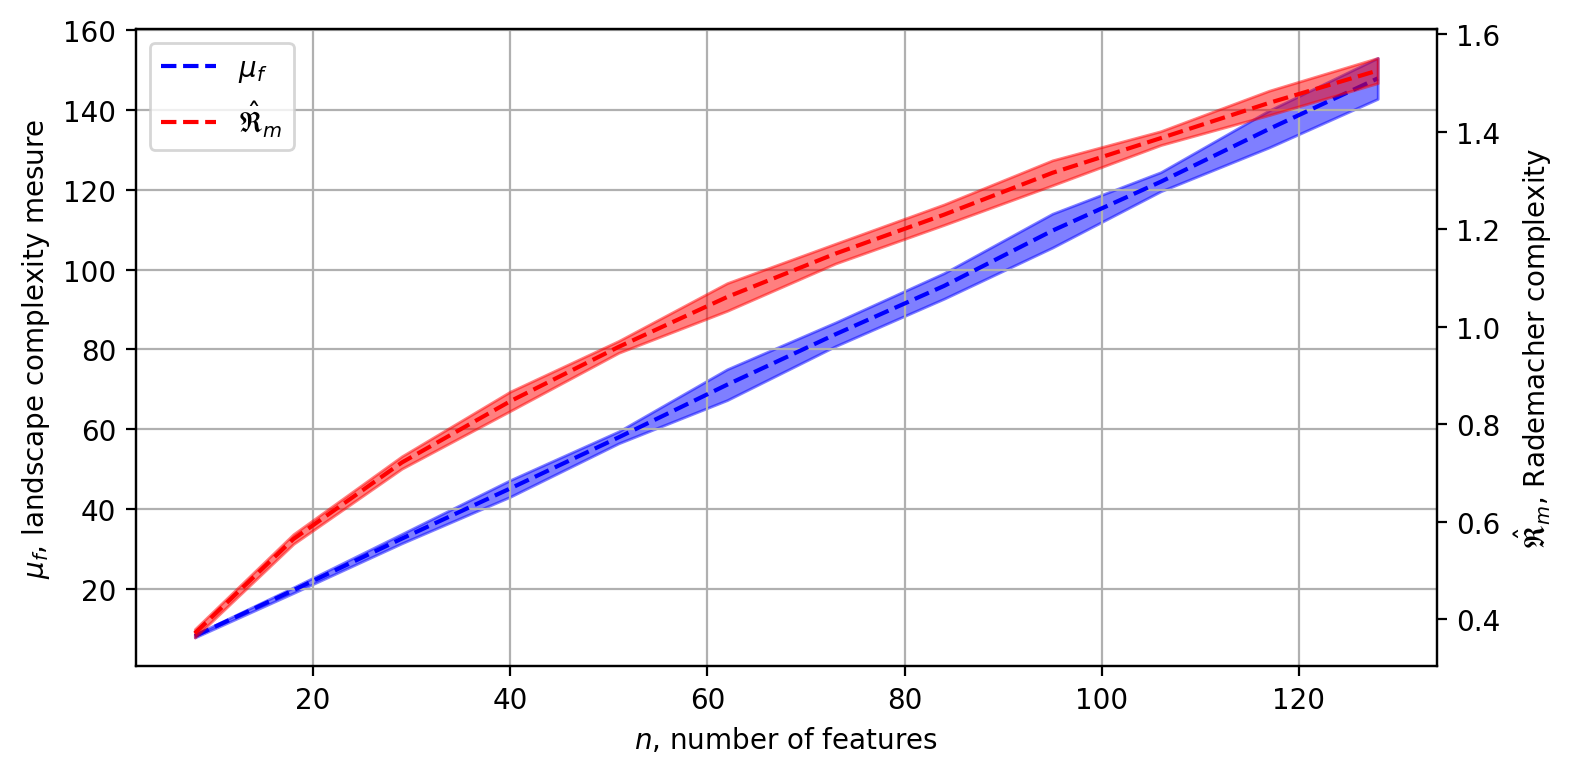
\includegraphics[width=0.62\linewidth]{../figures/exp01_linear_sweep_n.png}
\caption{Linear class: $\mu_f$ (left axis) and empirical $\hat{\mathfrak{R}}_m$ (right axis) versus ambient dimension~$n$ at fixed sample size $m=256$ and $W=2$. Shaded bands: mean $\pm$ std.\ over $16$ trials.}
\label{fig:exp01}
\end{figure}

\paragraph{Linear model, sweep in $m$ (fixed $n$).}
The setup fixes $n=64$ and varies $m$ on a geometric grid from $16$ to $1024$ with 14 values; targets use the same noise level as in the $n$-sweep.
Again, the experiment uses $W=2$ and $16$ trials per~$m$.
Figure~\ref{fig:exp02} shows the sweep in two panels. Panel~(a) plots $\mu_f$ versus~$m$. When the row norms of $\mathbf{x}_i$ stay stable as $m$ changes, $\mu_f$ also changes only weakly. This agrees with $\mu_f\le 2\max_i\|\mathbf{x}_i\|_2^2$ in~\eqref{eq:muf-lin-mu}. Panel~(b) plots $\hat{\mathfrak{R}}_m$ on log--log axes. It also shows a reference decay $\propto m^{-1/2}$, which illustrates the $m^{-1/2}$ factor in~\eqref{eq:Rad-lin-bound}.

\begin{figure}[t]
\centering
\begin{subfigure}[t]{0.48\textwidth}
\centering
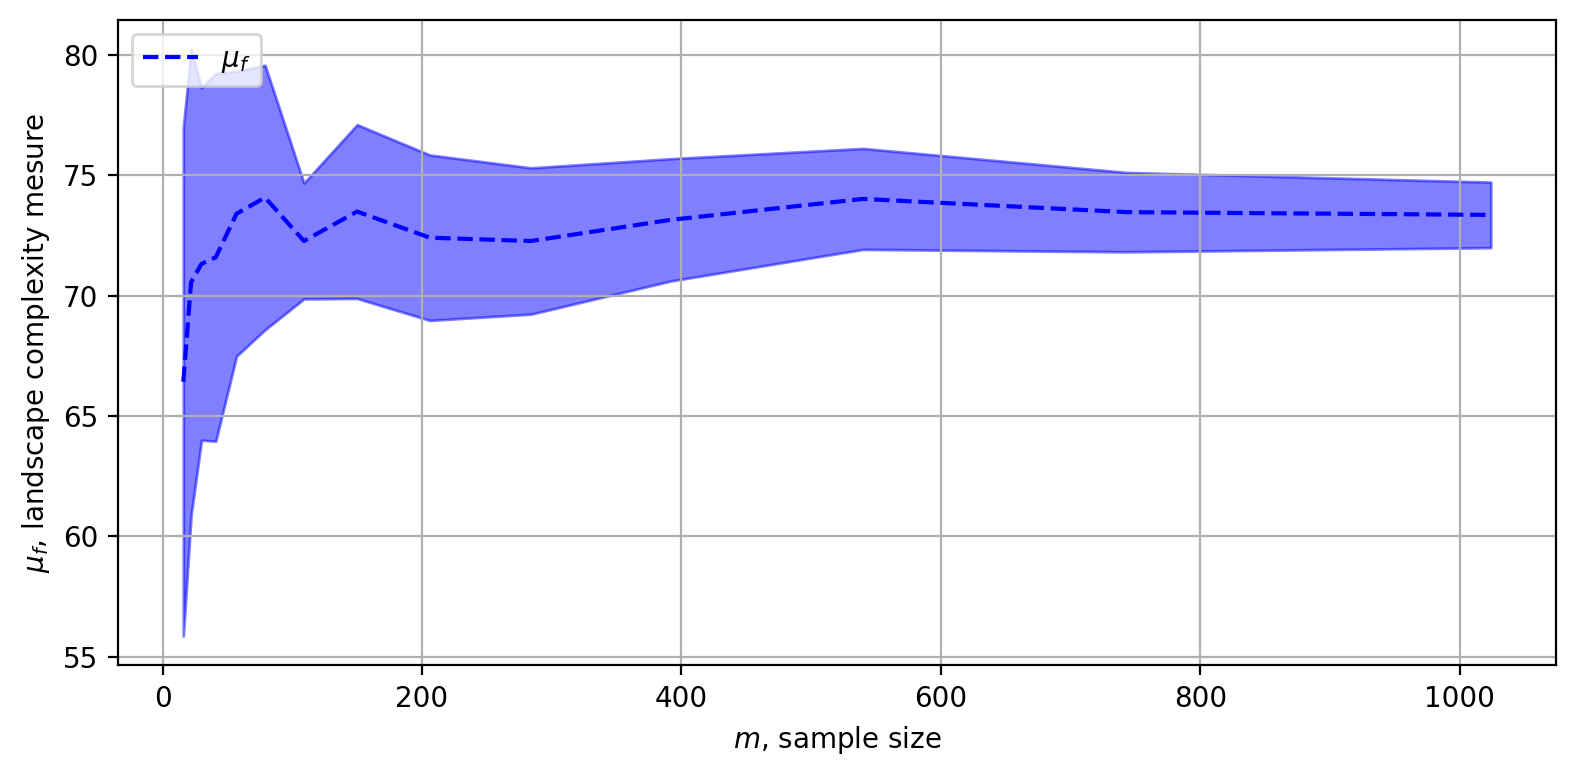
\includegraphics[width=\linewidth]{../figures/exp02_linear_sweep_m_mu.png}
\caption{$\mu_f$ vs.\ $m$.}
\label{fig:exp02-mu}
\end{subfigure}\hfill
\begin{subfigure}[t]{0.48\textwidth}
\centering
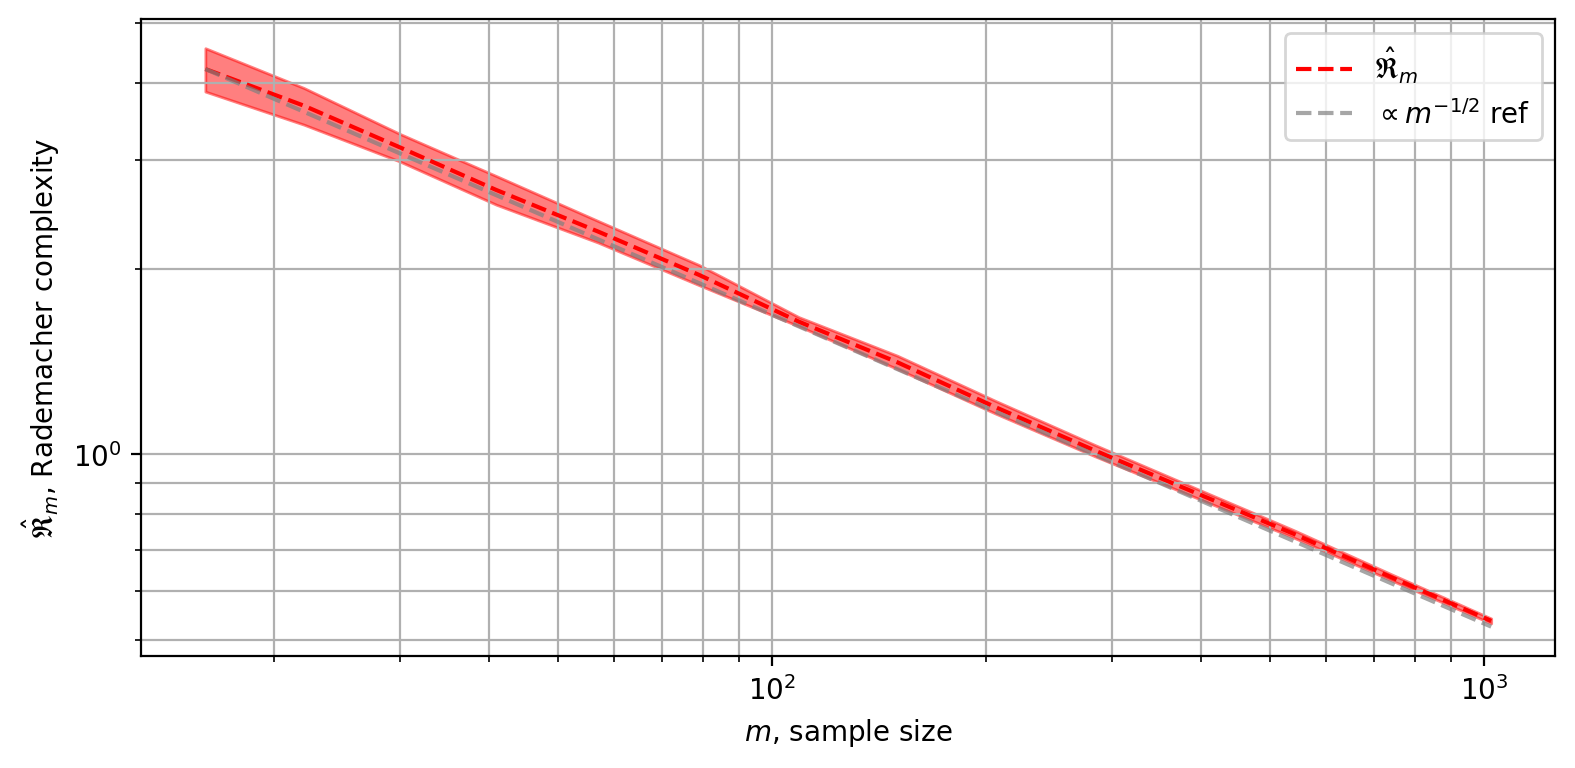
\includegraphics[width=\linewidth]{../figures/exp02_linear_sweep_m_rademacher.png}
\caption{$\hat{\mathfrak{R}}_m$ vs.\ $m$ (log--log).}
\label{fig:exp02-rad}
\end{subfigure}
\caption{Linear class, sweep in sample size~$m$ at fixed $n=64$ and $W=2$. Shaded bands: mean $\pm$ std.\ over $16$ trials; (b)~includes a dashed $\propto m^{-1/2}$ reference.}
\label{fig:exp02}
\end{figure}

\paragraph{Two-layer FC ReLU, sweep in $h$.}
The experiment uses the entrywise-bounded aligned teacher and clustered inputs from the code. The input dimension is tied to the width, so $n=h$. The setup uses the entrywise weight bound $M=1$, the sample size $m=512$, and hidden widths $h\in\{4,8,12,16,24,32\}$.
Evaluation is performed at the planted parameter $\boldsymbol{\theta}^\star$, so there is no label noise. As a result, the residual-aware discussion in Section~\ref{sec:compare} applies.
The quantity $\mu_f$ is estimated with batched per-example Hessians, using chunk size $64$ in the implementation. The quantity $\hat{\mathfrak{R}}_m$ is estimated with entrywise PGD as in the notebook, with $n_{\sigma}=64$ PGD steps.
Figure~\ref{fig:exp03} overlays empirical $\mu_f$ with two reference curves aligned at the smallest~$h$. One is the worst-case spectral scaling $\propto (Mh)^4$. The other is the residual-aware Gauss--Newton scaling $\propto h^3$ for $n=h$ from Subsection~\ref{subsec:two-layer-comp}. The figure also shows $\hat{\mathfrak{R}}_m$ on a second log axis so that its scale is not compressed by the larger values of~$\mu_f$.

\begin{figure}[t]
\centering
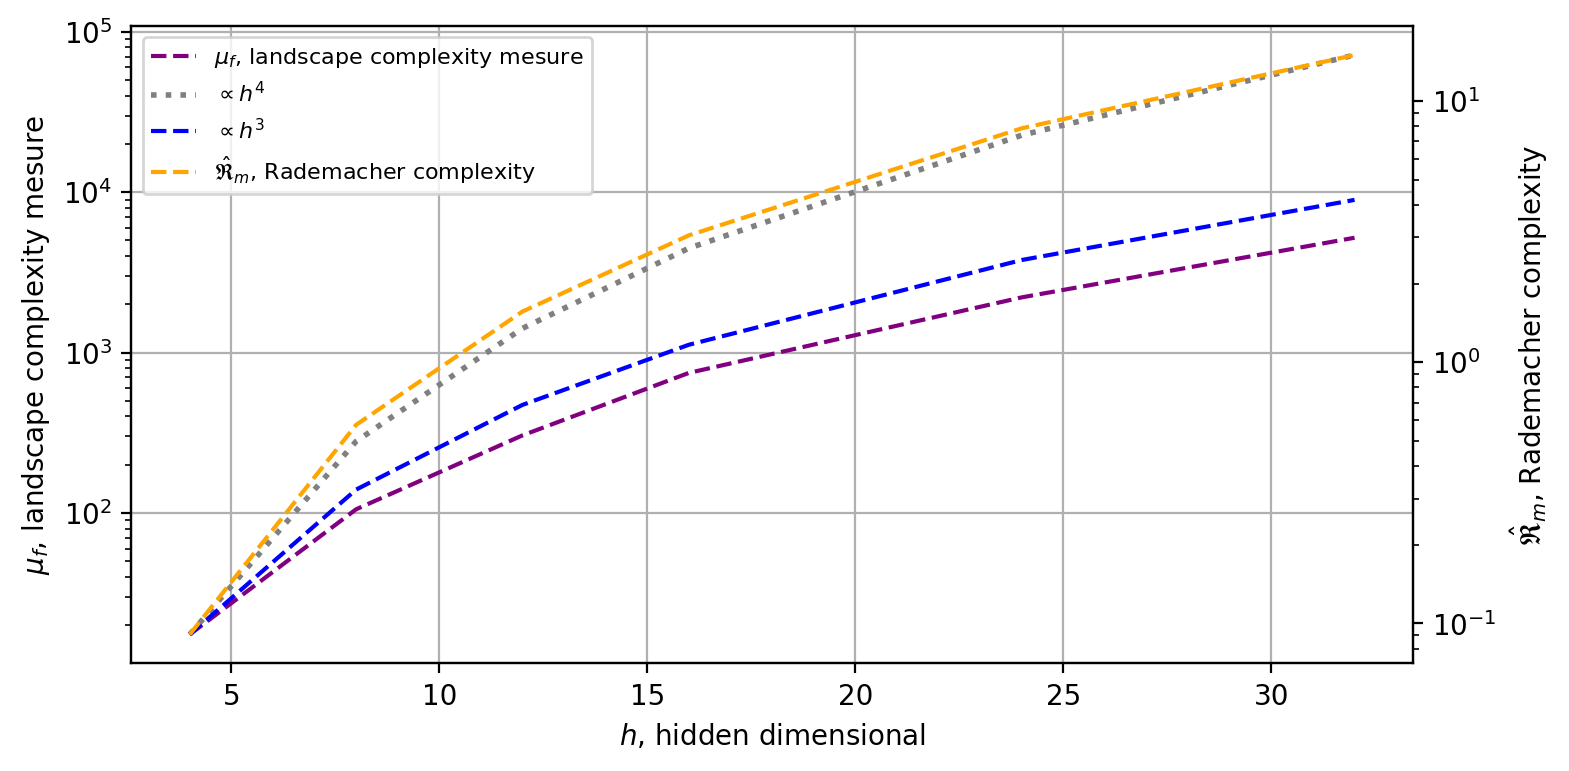
\includegraphics[width=0.62\linewidth]{../figures/exp03_twolayer_sweep_h.png}
\caption{Two-layer FC ReLU (entrywise bound $M=1$, $n=h$, planted optimum): empirical $\mu_f$ (left axis, log) with worst-case $\propto(Mh)^4$ and residual-aware GN $\propto h^3$ references; empirical $\hat{\mathfrak{R}}_m$ (right axis, log). Mean over $3$ random trials per~$h$.}
\label{fig:exp03}
\end{figure}

\section{Discussion}\label{sec:discussion}

Table~\ref{tab:compare-two} should be read as a comparison of two different notions of complexity. It should not be read as two upper bounds for the same phenomenon. Under the input-scaling assumptions of Subsection~\ref{subsec:linear-comp} and the norm assumptions of Lemma~\ref{lem:hess-mse}, the Landscape Complexity Measure reflects how strongly per-example Hessians vary around their empirical average at a fixed reference parameter. In the linear model, this gives an upper estimate that is \emph{linear} in the ambient dimension~$n$. In the worst-case two-layer ReLU regime, the same mechanism gives a \emph{quartic} upper estimate in the hidden width~$h$. The residual-aware part of Theorem~\ref{thm:landscape-mse} is also important. It shows that this worst-case picture is not the only one possible under squared loss. When residuals are small, the residual-weighted term in the per-example Hessian is suppressed. Then the Landscape Complexity Measure can scale more mildly. This refinement is local in nature and should be read in that same local sense throughout the comparison.

Empirical Rademacher complexity plays a different role. The bounds in~\eqref{eq:Rad-lin-bound} and~\eqref{eq:Rad-nn-generic} keep the common $m^{-1/2}$ decay in sample size. This happens because they measure global capacity of the predictor class rather than local curvature at one parameter. The architecture-dependent factor changes instead. In the linear case, it is of order $\sqrt{n}$. In the two-layer case, it is $O(\mathrm{poly}(h))$ under standard norm constraints. This is the main conceptual contrast of the paper. The Landscape Complexity Measure is sensitive to local Hessian variability and therefore to the chosen loss, reference point, and residual regime. In contrast, $\hat{\mathfrak{R}}_m$ is tied to the size of the real-valued function class. The loss-specific simplification $\|\mathbf{A}_{\mathrm{sq}}\|_2=1$ versus $\|\mathbf{A}_{\mathrm{CE}}\|_2\le\sqrt{2}$ makes this distinction especially clear. Changing the loss directly changes the Hessian-based landscape quantity through $\|\mathbf{H}_i\|_2$ and the outer factor $\|\mathbf{A}\|_2$. The Rademacher term remains attached to the function class itself rather than to that outer block~\cite{kiselev2024hessian}.

\section{Conclusion}\label{sec:conclusion}

This paper develops the Landscape Complexity Measure for scalar regression with fully connected ReLU networks under squared loss. It studies this quantity in linear and two-layer settings. For bias-free, norm-bounded networks, the paper adapts prior fully connected Hessian bounds to the MSE regime. It also identifies the simplification $\|\mathbf{A}_{\mathrm{sq}}\|_2=1$ relative to the softmax case. This leads to scaling laws for the proposed measure in terms of depth, width, and norm constraints.

The comparison with empirical Rademacher complexity shows that the two quantities are complementary rather than interchangeable. The numerical experiments are qualitatively consistent with this distinction and with the scaling trends derived in the theory.

Possible extensions include deeper architectures, broader input models, and regimes with non-negligible residuals. In such regimes, the residual-aware part of the Hessian bounds should become more prominent. The main contribution of the paper is the development of the Landscape Complexity Measure itself as a distinct complexity notion for squared-loss regression.

\begin{thebibliography}{99}

\bibitem{bartlett2002}
P.~L. Bartlett and S.~Mendelson.
\newblock Rademacher and Gaussian complexities: Risk bounds and structural results.
\newblock \emph{Journal of Machine Learning Research}, 3:463--482, 2002.

\bibitem{vapnik1998}
V.~N. Vapnik.
\newblock \emph{Statistical Learning Theory}.
\newblock Wiley, New York, 1998.

\bibitem{fort2019emergent}
S.~Fort and S.~Ganguli.
\newblock Emergent properties of the local geometry of neural loss landscapes.
\newblock arXiv:1910.05929, 2019.

\bibitem{ghorbani2019}
B.~Ghorbani, S.~Krishnan, and Y.~Xiao.
\newblock An investigation into neural net optimization via Hessian eigenvalue density.
\newblock In \emph{Proc.\ 36th Int.\ Conf.\ Machine Learning}, volume~97 of \emph{Proc.\ Mach.\ Learn.\ Res.}, pages 2232--2241. PMLR, 2019.

\bibitem{sagun2018}
L.~Sagun, U.~Evci, V.~U.~G{\"u}ney, Y.~Dauphin, and L.~Bottou.
\newblock Empirical analysis of the Hessian of over-parametrized neural networks.
\newblock arXiv:1706.04454, 2018.

\bibitem{pennington2017}
J.~Pennington and Y.~Bahri.
\newblock Geometry of neural network loss surfaces via random matrix theory.
\newblock In \emph{Proc.\ 34th Int.\ Conf.\ Machine Learning}, volume~70 of \emph{Proc.\ Mach.\ Learn.\ Res.}, pages 2798--2806. PMLR, 2017.

\bibitem{harvey2019jmlr}
P.~L. Bartlett, N.~Harvey, C.~Liaw, and A.~Mehrabian.
\newblock Nearly-tight VC-dimension and pseudodimension bounds for piecewise linear neural networks.
\newblock \emph{Journal of Machine Learning Research}, 20(63):1--17, 2019.
\newblock \href{https://jmlr.org/papers/v20/17-612.html}{\texttt{jmlr.org/papers/v20/17-612.html}}.

\bibitem{kiselev2024hessian}
N.~S. Kiselev and A.~V. Grabovoy.
\newblock Unraveling the {H}essian: {A} Key to Smooth Convergence in Loss Function Landscapes.
\newblock \emph{Doklady Mathematics}, 110(Suppl.~1):S49--S61, 2024.
\newblock \href{https://doi.org/10.1134/S1064562424601987}{\texttt{doi:10.1134/S1064562424601987}}.

\bibitem{choromanska2015}
A.~Choromanska, M.~Henaff, M.~Mathieu, G.~Ben~Arous, and Y.~LeCun.
\newblock The loss surfaces of multilayer networks.
\newblock In \emph{Proc.\ 18th Int.\ Conf.\ Artificial Intelligence and Statistics}, volume~38 of \emph{Proc.\ Mach.\ Learn.\ Res.}, pages 192--204. PMLR, 2015.

\bibitem{li2018visualizing}
H.~Li, Z.~Xu, G.~Taylor, C.~Studer, and T.~Goldstein.
\newblock Visualizing the loss landscape of neural nets.
\newblock In \emph{Advances in Neural Information Processing Systems}, volume~31, pages 6389--6399, 2018.

\bibitem{fort2019large}
S.~Fort and S.~Jastrzebski.
\newblock Large scale structure of neural network loss landscapes.
\newblock In \emph{Advances in Neural Information Processing Systems}, volume~32, 2019.

\bibitem{papyan2019hessian}
V.~Papyan.
\newblock The full spectrum of deepnet Hessians at scale: Dynamics with SGD training and sample size.
\newblock arXiv:1811.07062, 2019.

\bibitem{wu2022dissecting}
Y.~Wu, X.~Zhu, C.~Wu, A.~Wang, and R.~Ge.
\newblock Dissecting Hessian: Understanding common structure of Hessian in neural networks.
\newblock arXiv:2010.04261, 2022.

\bibitem{xie2022powerlaw}
Z.~Xie, Q.-Y.~Tang, Y.~Cai, M.~Sun, and P.~Li.
\newblock On the power-law Hessian spectrums in deep learning.
\newblock arXiv:2201.13011, 2022.

\bibitem{hochreiter1994}
S.~Hochreiter and J.~Schmidhuber.
\newblock Simplifying neural nets by discovering flat minima.
\newblock In \emph{Advances in Neural Information Processing Systems}, volume~7, pages 661--671. MIT Press, 1995.

\bibitem{neyshabur2017exploring}
B.~Neyshabur, S.~Bhojanapalli, D.~McAllester, and N.~Srebro.
\newblock Exploring generalization in deep learning.
\newblock arXiv:1706.08947, 2017.

\bibitem{dinh2017sharp}
L.~Dinh, R.~Pascanu, S.~Bengio, and Y.~Bengio.
\newblock Sharp minima can generalize for deep nets.
\newblock In \emph{Proc.\ 34th Int.\ Conf.\ Machine Learning}, volume~70 of \emph{Proc.\ Mach.\ Learn.\ Res.}, pages 1019--1028. PMLR, 2017.

\bibitem{singh2024lmc}
S.~P. Singh, L.~Adilova, M.~Kamp, A.~Fischer, B.~Sch{\"o}lkopf, and T.~Hofmann.
\newblock Landscaping linear mode connectivity.
\newblock arXiv:2406.16300, 2024.

\bibitem{singh2022double}
S.~P. Singh, A.~Lucchi, T.~Hofmann, and B.~Sch{\"o}lkopf.
\newblock Phenomenology of double descent in finite-width neural networks.
\newblock arXiv:2203.07337, 2022.

\bibitem{meshkov2024ispras}
V.~Meshkov, N.~Kiselev, and A.~Grabovoy.
\newblock {ConvNets} landscape convergence: {H}essian-based analysis of matricized networks.
\newblock In \emph{2024 Ivannikov Ispras Open Conference (ISPRAS)}, pages 1--10. IEEE, 2024.
\newblock \href{https://doi.org/10.1109/ispras64596.2024.10899113}{\texttt{doi:10.1109/ispras64596.2024.10899113}}.

\bibitem{jacot2018ntk}
A.~Jacot, F.~Gabriel, and C.~Hongler.
\newblock Neural tangent kernel: Convergence and generalization in neural networks.
\newblock In \emph{Advances in Neural Information Processing Systems}, volume~31, 2018.

\bibitem{lee2018wide}
J.~Lee, L.~Xiao, S.~S. Schoenholz, Y.~Bahri, R.~Novak, J.~Sohl-Dickstein, and J.~Pennington.
\newblock Wide neural networks of any depth evolve as linear models under gradient descent.
\newblock \emph{J.\ Stat.\ Mech.\ Theory Exp.}, 2020(12):124002, 2020.

\bibitem{skorski2019chain}
M.~Skorski.
\newblock Chain rules for Hessian and higher derivatives made easy by tensor calculus.
\newblock arXiv:1911.13292, 2019.

\end{thebibliography}

\appendix

\section{Proofs}

\subsection{Second-order approximation motivating~\eqref{eq:mod-diff}}\label{app:proof-mod-diff}

Write $\boldsymbol{\delta}=\boldsymbol{\theta}-\boldsymbol{\theta}^*$.
Under Assumption~\ref{ass:local-min}, and on regions where the relevant derivatives exist, the second-order approximations read
\[
  \mathcal{L}_k(\boldsymbol{\theta})
  \approx \mathcal{L}_k(\boldsymbol{\theta}^*)
  + \nabla\mathcal{L}_k(\boldsymbol{\theta}^*)^\top\boldsymbol{\delta}
  + \tfrac{1}{2}\boldsymbol{\delta}^\top \mathbf{H}^{(k)}(\boldsymbol{\theta}^*)\boldsymbol{\delta},
\]
Here $\mathbf{H}^{(k)}(\boldsymbol{\theta}^*)=\frac{1}{k}\sum_{i=1}^k \mathbf{H}_i(\boldsymbol{\theta}^*)$. An analogous formula holds for $\mathcal{L}_{k+1}$. Subtracting the two expressions gives
\begin{align*}
  \mathcal{L}_{k+1}(\boldsymbol{\theta}) - \mathcal{L}_k(\boldsymbol{\theta})
  &\approx \mathcal{L}_{k+1}(\boldsymbol{\theta}^*) - \mathcal{L}_k(\boldsymbol{\theta}^*)
  + \bigl(\nabla\mathcal{L}_{k+1}(\boldsymbol{\theta}^*) - \nabla\mathcal{L}_k(\boldsymbol{\theta}^*)\bigr)^\top\boldsymbol{\delta}
  \\
  &\quad + \tfrac{1}{2}\boldsymbol{\delta}^\top
  \Bigl(\mathbf{H}^{(k+1)}(\boldsymbol{\theta}^*) - \mathbf{H}^{(k)}(\boldsymbol{\theta}^*)\Bigr)\boldsymbol{\delta}.
\end{align*}
The zeroth-order difference $\mathcal{L}_{k+1}(\boldsymbol{\theta}^*) - \mathcal{L}_k(\boldsymbol{\theta}^*)$ equals
$\frac{1}{k+1}\bigl(\ell(f_{\boldsymbol{\theta}^*}(\mathbf{x}_{k+1}),\mathbf{y}_{k+1}) - \frac{1}{k}\sum_{i=1}^{k}\ell(f_{\boldsymbol{\theta}^*}(\mathbf{x}_{i}),\mathbf{y}_{i})\bigr)$.
If $\varepsilon_g=0$, the linear terms vanish. Then the quadratic contribution reduces to the form in \cite{kiselev2024hessian}. For $\varepsilon_g\ge 0$, the same modulus bounds apply to the quadratic term.
By Cauchy--Schwarz and~\eqref{eq:eps-g},
\[
  \bigl|\bigl(\nabla\mathcal{L}_{k+1}(\boldsymbol{\theta}^*) - \nabla\mathcal{L}_k(\boldsymbol{\theta}^*)\bigr)^\top\boldsymbol{\delta}\bigr|
  \le \bigl(\|\nabla\mathcal{L}_{k+1}(\boldsymbol{\theta}^*)\|_2 + \|\nabla\mathcal{L}_k(\boldsymbol{\theta}^*)\|_2\bigr)\|\boldsymbol{\delta}\|_2
  \le 2\varepsilon_g\|\boldsymbol{\delta}\|_2 .
\]
Combining with the triangle inequality and $|\mathbf{u}^\top \mathbf{M}\mathbf{u}|\le \|\mathbf{u}\|_2^2\|\mathbf{M}\|_2$ for the quadratic part leads to the local proxy estimate~\eqref{eq:mod-diff}.

\subsection{Proof of Lemma~\ref{lem:hess-mse}}\label{app:proof-lemma-hess}

Write $u_i=f_{\boldsymbol{\theta}}(\mathbf{x}_i)$ and $\ell(u,y)=\tfrac{1}{2}(u-y)^2$. The Hessian decomposition for scalar output is as follows.
For a $K$-dimensional logit vector $\mathbf{z}$, \cite{kiselev2024hessian} (Section~3.4) decompose
\[
  \mathbf{H}_i(\boldsymbol{\theta})
  = \nabla_{\boldsymbol{\theta}}\mathbf{z}_i\,\frac{\partial^2\ell}{\partial\mathbf{z}_i^2}\,\nabla_{\boldsymbol{\theta}}\mathbf{z}_i^{\top}
  + \sum_{k=1}^{K}\frac{\partial\ell}{\partial z_{ik}}\,\nabla_{\boldsymbol{\theta}}^2 z_{ik}.
\]
Here $K=1$, $\mathbf{z}_i=u_i\in\mathbb{R}$, $\partial^2\ell/\partial u_i^2=1$, and $\partial\ell/\partial u_i=u_i-y_i$, hence
\begin{equation}\label{eq:hess-mse-decomp}
  \mathbf{H}_i(\boldsymbol{\theta})
  = \nabla_{\boldsymbol{\theta}}u_i\,\nabla_{\boldsymbol{\theta}}u_i^{\top}
  + (u_i-y_i)\,\nabla_{\boldsymbol{\theta}}^2 u_i .
\end{equation}
Thus the first summand is rank one, and its spectral norm is $\|\nabla_{\boldsymbol{\theta}}u_i\|_2^2$. The second summand is the network Hessian weighted by the residual.
For softmax cross-entropy, $\partial^2\ell/\partial\mathbf{z}^2=\mathrm{diag}(\mathbf{p})-\mathbf{p}\mathbf{p}^{\top}$ and $\|\partial^2\ell/\partial\mathbf{z}^2\|_2\le\sqrt{2}$ \cite{kiselev2024hessian}; that factor $\sqrt{2}$ is the one that appears in Theorem~1 there.

From~\eqref{eq:hess-mse-decomp} and the triangle inequality, the following pointwise spectral bound is obtained:
\begin{equation}\label{eq:hess-mse-triangle}
  \bigl\|\mathbf{H}_i(\boldsymbol{\theta})\bigr\|_2
  \le \bigl\|\nabla_{\boldsymbol{\theta}}u_i\bigr\|_2^2
  + |u_i-y_i|\,\bigl\|\nabla_{\boldsymbol{\theta}}^2 u_i\bigr\|_2 .
\end{equation}
This isolates the residual $|u_i-y_i|$ in the second term. By contrast, Lemma~\ref{lem:hess-mse} records a \emph{uniform} majorant of the form~\eqref{eq:Mh-bound}. This majorant is obtained by specializing the fully connected analysis in \cite{kiselev2024hessian}, Theorem~1 and Appendix~A.2, from $K$-way softmax to scalar output and squared loss.

Theorem~1 of \cite{kiselev2024hessian} states, for their cross-entropy setup,
\[
  \|\mathbf{H}_i(\boldsymbol{\theta})\|_2
  \le L\sqrt{2}\,M_{\mathbf{x}}^2 M_{\mathbf{W}}^{2L}
  + \sqrt{2}\,\frac{M_{\mathbf{W}}^2\bigl(M_{\mathbf{W}}^{2L}-1\bigr)}{M_{\mathbf{W}}^2-1}.
\]
Their Appendix~A.2 derives this closed form under $\|\mathbf{W}^{(p)}\|_2\le M_{\mathbf{W}}$ and $\|\mathbf{x}_i\|_2\le M_{\mathbf{x}}$. The prefactors $\sqrt{2}$ match the spectral norm of the softmax loss Hessian $\|\partial^2\ell/\partial\mathbf{z}^2\|_2\le\sqrt{2}$.
For scalar output and squared loss, the outer Hessian is the scalar $\partial^2\ell/\partial u^2=1$. The Jacobian $\nabla_{\boldsymbol{\theta}}\mathbf{z}_i$ then reduces to the column $\nabla_{\boldsymbol{\theta}}u_i$. In this specialization, the softmax-loss factor $\sqrt{2}$ is replaced by~$1$. The remaining dependence on $L$, $M_{\mathbf{x}}$, and $M_{\mathbf{W}}$ stays the same. Writing the second term as the equivalent finite sum $\sum_{s=1}^{L} M_{\mathbf{W}}^{2s}$ avoids the removable singularity at $M_{\mathbf{W}}=1$ and yields~\eqref{eq:Mh-bound}.

Identity~\eqref{eq:hess-mse-decomp} is exact; \eqref{eq:hess-mse-triangle} is a pointwise inequality.
The closed form~\eqref{eq:Mh-bound} is the MSE counterpart of \cite{kiselev2024hessian}, Theorem~1, and is not claimed to be sharp in $|u_i-y_i|$ (cf.~\eqref{eq:hess-mse-triangle}).
If $|w_{ij}^{(p)}|\le M$ on $h\times h$ blocks, then $M_{\mathbf{W}}\le hM$ and $\|\mathbf{H}_i\|_2=O(L(hM)^{2L})$ asymptotically.

\subsection{Proof of Theorem~\ref{thm:landscape-mse}}\label{app:proof-thm-landscape}

Assume the local proxy estimate~\eqref{eq:mod-diff}. The first term is bounded first:
\[
  \Bigl|\ell(f_{\boldsymbol{\theta}^*}(\mathbf{x}_{k+1}),\mathbf{y}_{k+1}) - \frac{1}{k}\sum_{i=1}^{k}\ell(f_{\boldsymbol{\theta}^*}(\mathbf{x}_{i}),\mathbf{y}_{i})\Bigr|
  \le \bigl|\ell(f_{\boldsymbol{\theta}^*}(\mathbf{x}_{k+1}),\mathbf{y}_{k+1})\bigr|
  + \frac{1}{k}\sum_{i=1}^{k}\bigl|\ell(f_{\boldsymbol{\theta}^*}(\mathbf{x}_{i}),\mathbf{y}_{i})\bigr|
  \le 2M_{\ell},
\]
using $\bigl|\ell(f_{\boldsymbol{\theta}^*}(\mathbf{x}_{i}),\mathbf{y}_i)\bigr|\le M_{\ell}$ for each $i$.
For the Hessian difference, the triangle inequality gives
\[
  \left\| \mathbf{H}_{k+1}(\boldsymbol{\theta}^*) - \frac{1}{k}\sum_{i=1}^{k}\mathbf{H}_i(\boldsymbol{\theta}^*) \right\|_2
  \le \|\mathbf{H}_{k+1}(\boldsymbol{\theta}^*)\|_2 + \frac{1}{k}\sum_{i=1}^{k}\|\mathbf{H}_i(\boldsymbol{\theta}^*)\|_2
  \le 2M_{\mathbf{H}},
\]
since $\|\mathbf{H}_i(\boldsymbol{\theta}^*)\|_2\le M_{\mathbf{H}}$ for all $i$ by Lemma~\ref{lem:hess-mse}.
Now substitute into~\eqref{eq:mod-diff}. Also use $\|\boldsymbol{\theta}-\boldsymbol{\theta}^*\|_2\le R$ and $\|\boldsymbol{\theta}-\boldsymbol{\theta}^*\|_2^2\le R^2$:
\[
  \bigl|\mathcal{L}_{k+1}(\boldsymbol{\theta}) - \mathcal{L}_k(\boldsymbol{\theta})\bigr|
  \le \frac{2M_{\ell}}{k+1} + \frac{2M_{\mathbf{H}}R^2}{k+1} + 2\varepsilon_g R
  = \frac{2}{k+1}\bigl(M_{\ell} + M_{\mathbf{H}}R^2\bigr) + 2\varepsilon_g R ,
\]
which is~\eqref{eq:thm-bound}. The rate~\eqref{eq:rate} follows for $\varepsilon_g=0$ by substituting the asymptotic upper bound
$M_{\mathbf{H}}=O(L(hM)^{2L})$ from Lemma~\ref{lem:hess-mse}.

Assume now $\bigl|f_{\boldsymbol{\theta}^*}(\mathbf{x}_i)-y_i\bigr|\le \varepsilon_y$ for every $i$ and define
$\mathbf{g}_i:=\nabla_{\boldsymbol{\theta}}f_{\boldsymbol{\theta}^*}(\mathbf{x}_i)$ and
$M_{\nabla^2 f}:=\max_i\|\nabla_{\boldsymbol{\theta}}^2f_{\boldsymbol{\theta}^*}(\mathbf{x}_i)\|_2$.
Then~\eqref{eq:hess-mse-decomp} gives
\[
  \mathbf{H}_i(\boldsymbol{\theta}^*)
  = \mathbf{g}_i\mathbf{g}_i^\top
  + \bigl(f_{\boldsymbol{\theta}^*}(\mathbf{x}_i)-y_i\bigr)\nabla_{\boldsymbol{\theta}}^2 f_{\boldsymbol{\theta}^*}(\mathbf{x}_i),
\]
hence
\[
  \bigl\|
    \mathbf{H}_i(\boldsymbol{\theta}^*)
    - \mathbf{g}_i\mathbf{g}_i^\top
  \bigr\|_2
  \le \varepsilon_y M_{\nabla^2 f},
\]
which is~\eqref{eq:interp-hessian}.

Let $\bar{\mathbf{H}}:=\frac{1}{m}\sum_{j=1}^{m}\mathbf{H}_j(\boldsymbol{\theta}^*)$ and
$\bar{\mathbf{G}}:=\frac{1}{m}\sum_{j=1}^{m}\mathbf{g}_j\mathbf{g}_j^\top$.
Then
\begin{align*}
  \|\mathbf{H}_i(\boldsymbol{\theta}^*)-\bar{\mathbf{H}}\|_2
  &\le \|\mathbf{g}_i\mathbf{g}_i^\top-\bar{\mathbf{G}}\|_2
    + \bigl\|\mathbf{H}_i(\boldsymbol{\theta}^*)-\mathbf{g}_i\mathbf{g}_i^\top\bigr\|_2
    + \|\bar{\mathbf{H}}-\bar{\mathbf{G}}\|_2 \\
  &\le \|\mathbf{g}_i\|_2^2 + \frac{1}{m}\sum_{j=1}^{m}\|\mathbf{g}_j\|_2^2
    + \varepsilon_y M_{\nabla^2 f}
    + \frac{1}{m}\sum_{j=1}^{m}\bigl\|\mathbf{H}_j(\boldsymbol{\theta}^*)-\mathbf{g}_j\mathbf{g}_j^\top\bigr\|_2 \\
  &\le 2\max_{1\le j\le m}\|\mathbf{g}_j\|_2^2 + 2\varepsilon_y M_{\nabla^2 f},
\end{align*}
because $\|\mathbf{g}_i\mathbf{g}_i^\top\|_2=\|\mathbf{g}_i\|_2^2$ and $\|\cdot\|_2$ is convex.
Averaging over $i$ yields~\eqref{eq:muf-interp-general}.

Now return to~\eqref{eq:mod-diff}. Since $\ell_i(\boldsymbol{\theta}^*)=\tfrac12(f_{\boldsymbol{\theta}^*}(\mathbf{x}_i)-y_i)^2\le \tfrac12\varepsilon_y^2$ for all $i$,
its zeroth-order term is at most $\varepsilon_y^2/(k+1)$.
For the quadratic term,
\[
  \left\| \mathbf{H}_{k+1}(\boldsymbol{\theta}^*) - \frac{1}{k}\sum_{i=1}^{k}\mathbf{H}_i(\boldsymbol{\theta}^*) \right\|_2
  \le 2\max_{1\le i\le m}\|\mathbf{g}_i\|_2^2 + 2\varepsilon_y M_{\nabla^2 f},
\]
by the same averaging argument on the first $k+1$ samples.
Substituting into~\eqref{eq:mod-diff} gives~\eqref{eq:thm-bound-interp}.

It remains to prove~\eqref{eq:grad-interp-general}.
Write the forward activations as $\mathbf{a}^{(0)}=\mathbf{x}_i$,
$\mathbf{a}^{(p)}=\sigma(\mathbf{W}^{(p)\star}\mathbf{a}^{(p-1)})$ for $p=1,\dots,L-1$, and
$f_{\boldsymbol{\theta}^*}(\mathbf{x}_i)=\mathbf{W}^{(L)\star}\mathbf{a}^{(L-1)}$.
Since ReLU is $1$-Lipschitz and positively homogeneous,
\[
  \|\mathbf{a}^{(p)}\|_2 \le M_{\mathbf{W}}^{p}\|\mathbf{x}_i\|_2 \le M_{\mathbf{W}}^{p}M_{\mathbf{x}} .
\]
For the backpropagated derivatives $\boldsymbol{\delta}^{(L)}=1$ and
$\boldsymbol{\delta}^{(p)}=\mathbf{D}^{(p)}(\mathbf{W}^{(p+1)\star})^\top \boldsymbol{\delta}^{(p+1)}$ with diagonal ReLU masks $\mathbf{D}^{(p)}$ satisfying $\|\mathbf{D}^{(p)}\|_2\le 1$, one has
\[
  \|\boldsymbol{\delta}^{(p)}\|_2 \le M_{\mathbf{W}}^{L-p}.
\]
The gradient with respect to the layer-$p$ weights is
$\nabla_{\mathbf{W}^{(p)}} f_{\boldsymbol{\theta}^*}(\mathbf{x}_i)
 = \boldsymbol{\delta}^{(p)}(\mathbf{a}^{(p-1)})^\top$,
so its Frobenius norm satisfies
\[
  \left\|\nabla_{\mathbf{W}^{(p)}} f_{\boldsymbol{\theta}^*}(\mathbf{x}_i)\right\|_F
  \le \|\boldsymbol{\delta}^{(p)}\|_2\,\|\mathbf{a}^{(p-1)}\|_2
  \le M_{\mathbf{W}}^{L-p} M_{\mathbf{W}}^{p-1} M_{\mathbf{x}}
  = M_{\mathbf{x}} M_{\mathbf{W}}^{L-1}.
\]
Summing the squared Frobenius norms over $p=1,\dots,L$ gives
\[
  \bigl\|\nabla_{\boldsymbol{\theta}}f_{\boldsymbol{\theta}^*}(\mathbf{x}_i)\bigr\|_2^2
  = \sum_{p=1}^{L}\left\|\nabla_{\mathbf{W}^{(p)}} f_{\boldsymbol{\theta}^*}(\mathbf{x}_i)\right\|_F^2
  \le L M_{\mathbf{x}}^2 M_{\mathbf{W}}^{2L-2},
\]
which is~\eqref{eq:grad-interp-general}. Substituting this into~\eqref{eq:thm-bound-interp}
proves~\eqref{eq:rate-interp}.

\end{document}